\documentclass[UTF8]{ctexart}
\usepackage{subfigure}
\usepackage{caption}
\usepackage{amsmath}
\usepackage{geometry}
\usepackage{graphicx}
\usepackage{gensymb}
\usepackage{wrapfig}
\usepackage{titlesec}
\usepackage{float}
\usepackage{diagbox}
\usepackage{fancyhdr}
\pagestyle{plain}
\geometry{a4paper,scale=0.8}
\CTEXsetup[format+={\raggedright}]{section} 
\title{量统2017-2018郭永期末}
\author{Deschain}
\titlespacing*{\section}
{0pt}{0pt}{0pt}
\titlespacing*{\subsection}
{0pt}{0pt}{0pt}
\titlespacing*{\paragraph}
{0pt}{0pt}{0pt}
\titlespacing*{\subparagraph}
{0pt}{0pt}{0pt}
\titleformat*{\section}{\normalsize}
\begin{document}
\maketitle
\section*{一、(15分,每小题3分)简答题:解释下列概念:1.全同粒子2.玻尔兹曼关系3.等几率原理4.费米能5.$\mu$空间}
1.全同粒子:质量、电荷、自旋等内禀属性完全相同的粒子,具有不可区分性。\\
2.玻尔兹曼关系:$S=kln(W\{n_i\})$,S是熵,k是Boltzmann常数,$W\{n_i\}$是系统的微观状态数。\\
3.等几率原理:对于处于平衡态的孤立系统,各个微观态出现的几率相等。\\
4.费米能:在$T=0K$时,低于费米能的能级全被填满,高于费米能的能级全部空着。\\
5.$\mu$空间:以广义坐标和广义动量为直角坐标系基矢的$2r$维空间。
\section*{二、(本题20分)一个由大量全同和近独立的玻色子组成的孤立系统,具有确定粒子数N、能量E和体积V,
  设$\varepsilon_i,g_i,n_i$分别是单粒子能级i的能量、简并度和占有数。解答下列问题:}
1.写出该玻色系统中任意一组分布$\{n_i\}$所包含的微观状态数。
\begin{equation*}
  \begin{aligned}
    W\{n_i\}=\prod\limits_i\frac{(n_i+g_i-1)!}{n_i!(g_i-1)!}
  \end{aligned}
\end{equation*}
2.基于等几率原理并采用Lagrange待定乘子法,导出玻色-爱因斯坦分布
$n_i=\frac{g_i}{e^{\alpha+\beta\varepsilon_1}-1},(i=1,2,\cdots)$,
进而解释该分布的含义。
\begin{equation*}
  \begin{aligned}
     & W\{n_i\}=\prod\limits_i\frac{(n_i+g_i-1)!}{n_i!(g_i-1)!}                          \\
     & ln(W\{n_i\})\approx\sum(n_i+g_i)ln(n_i+g+i)-n_ilnn_i-g_ilng_i                     \\
     & F(n_i)=ln(W\{n_i\})+\alpha(N-\sum n_i)+\beta(E-\sum n_i\varepsilon_i)             \\
     & \frac{\partial F}{\partial n_i}=ln(1+\frac{g_i}{n_i})-\alpha-\beta\varepsilon_i=0 \\
     & n_i=\frac{g_i}{e^{\alpha+\beta\varepsilon_i}-1}
  \end{aligned}
\end{equation*}
3.直接给出玻色气体可以采用半经典近似$n_i=g_ie^{-\alpha-\beta\varepsilon_i}$的条件。
\begin{equation*}
  e^\alpha>>1
\end{equation*}
4.分别做出由玻色-爱因斯坦统计及费米-狄拉克统计所支配的近独立粒子系统在两不同温度时能级$\varepsilon$
上分布的粒子数随能级$\varepsilon$变化的草图。\\
参考公式:Stirling公式$N!\approx N^Ne^{-N}\quad(N>>1)$\\
\begin{figure}[H]
  \centering
  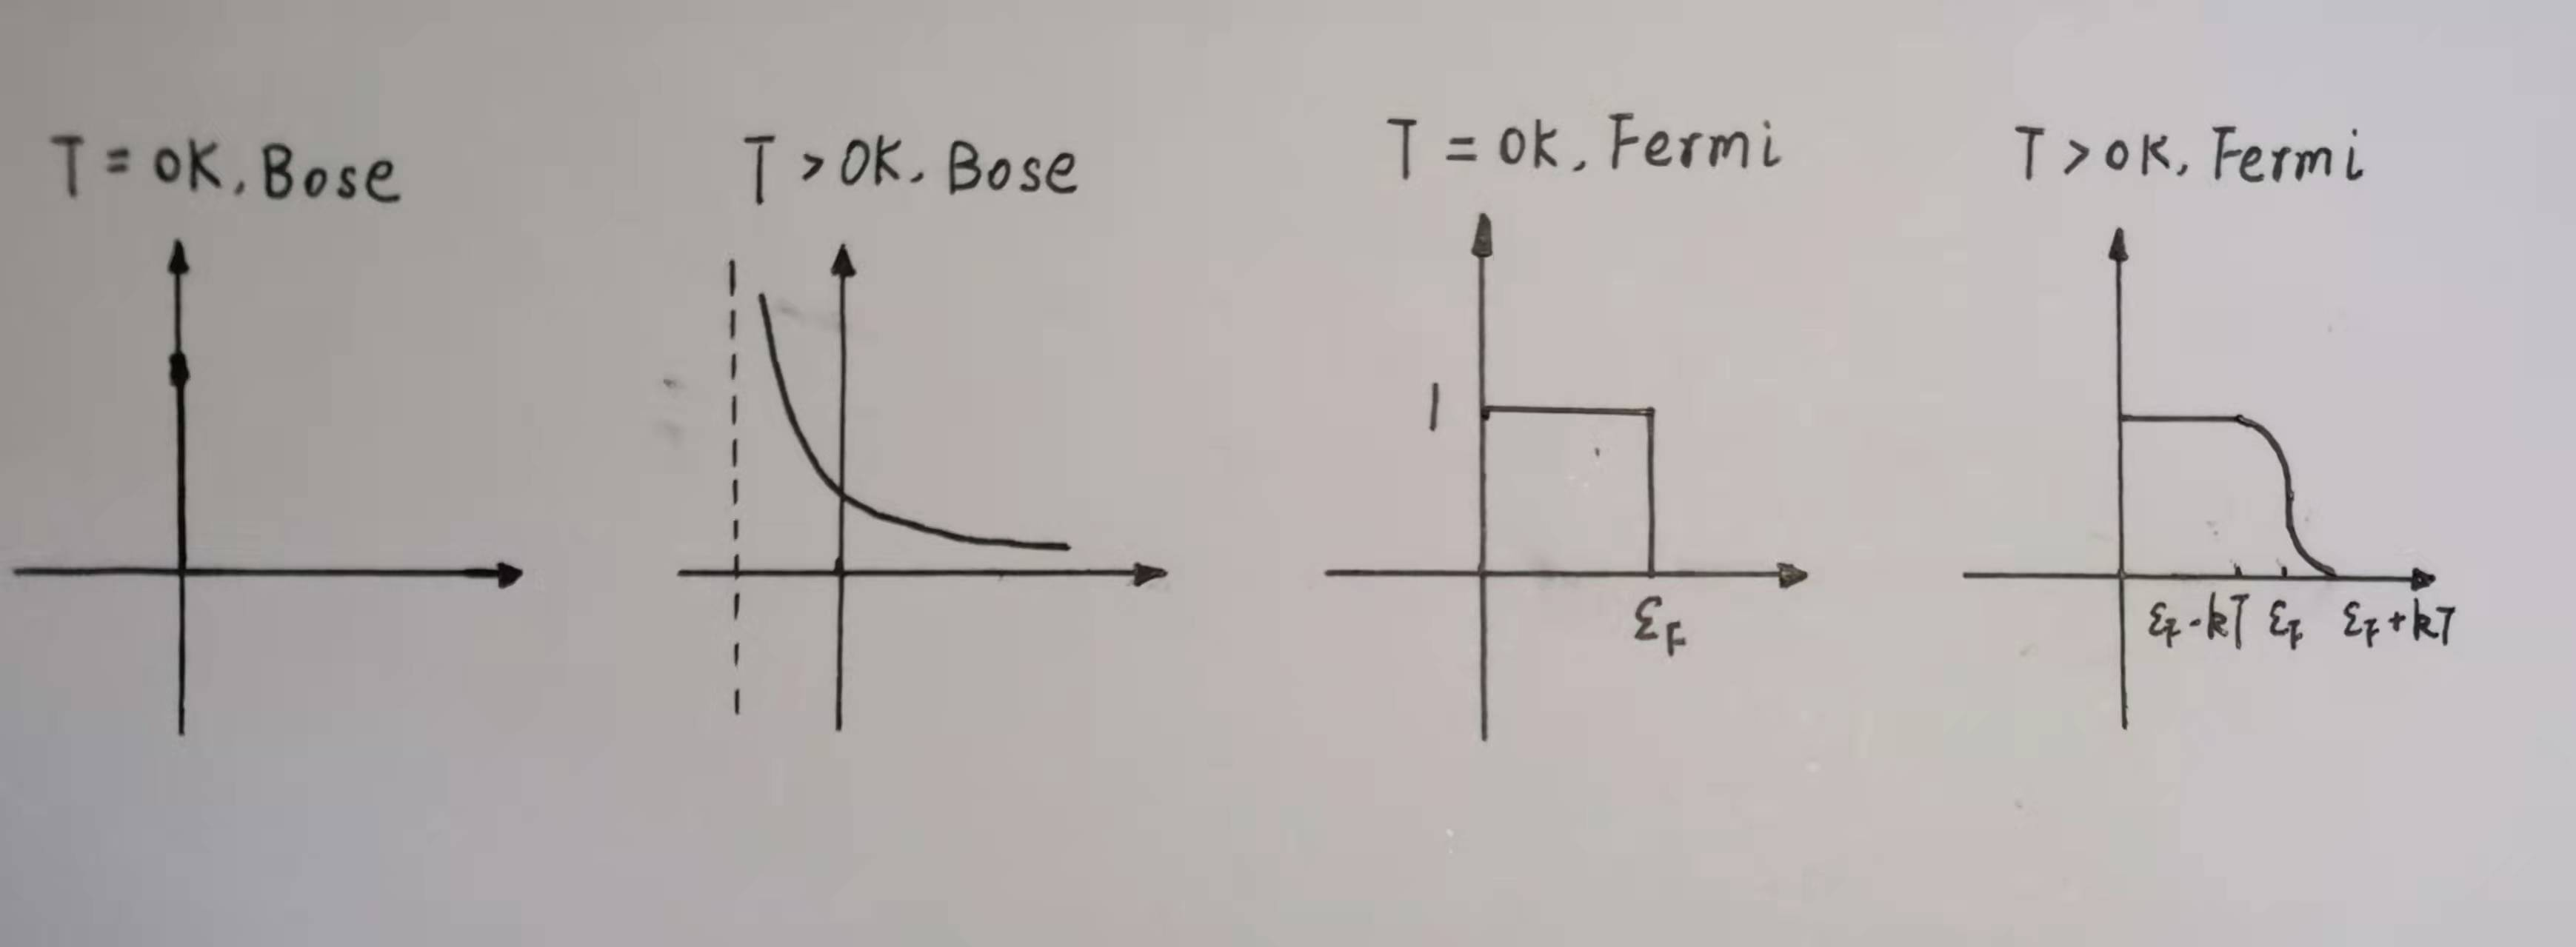
\includegraphics[width=12cm,height=3cm]{2_4.jpg}
\end{figure}
\section*{三、(本题20分)一定域系统含有N个近独立粒子,每个粒子有两个非简并能级
  $\varepsilon_0$和$\varepsilon_1(\varepsilon_1>\varepsilon_0)$,解答下列问题:}
1.在温度为T的热平衡状态下,粒子在能级$\varepsilon_0$和$\varepsilon_1$的粒子分布数。
\begin{equation*}
  \begin{aligned}
     & n_i=g_ie^{-\alpha-\beta\varepsilon_i},\quad g_0=g_1=1   \\
     & n_0=e^{-\alpha-\frac{\varepsilon_0}{kT}},
    \quad n_1=e^{-\alpha-\frac{\varepsilon_1}{kT}}             \\
     & n_0+n_1=N\quad\quad
    n_0=\frac{N}{1+e^{\frac{\varepsilon_0-\varepsilon_1}{kT}}},\quad
    n_1=\frac{N}{1+e^{\frac{\varepsilon_1-\varepsilon_0}{kT}}} \\
  \end{aligned}
\end{equation*}
2.在温度为T的热平衡状态下系统的内能、定容热容及熵;
\begin{equation*}
  \begin{aligned}
     & z = e^{-\beta\varepsilon_0}+e^{-\beta\varepsilon_1} \\
     & \overline{E}=-N\frac{\partial lnz}{\partial\beta}
    =N\frac{\varepsilon_0e^{-\beta\varepsilon_0}+\varepsilon_1e^{-\beta\varepsilon_1}}
    {e^{-\beta\varepsilon_0}+e^{-\beta\varepsilon_1}}      \\
     & C_V=(\frac{\partial\overline{E}}{\partial T})_V
    =\frac{N(\varepsilon_0-\varepsilon_1)}{kT^2}e^{\frac{\varepsilon_1-\varepsilon_0}{kT}}
    \frac{\varepsilon_0+
    (\varepsilon_0-\frac{\varepsilon_1(\varepsilon_0-\varepsilon_1)}{kT^2})
    e^{\frac{\varepsilon_1-\varepsilon_0}{kT^2}}
    -\frac{\varepsilon_0(\varepsilon_0-\varepsilon_1)}{kT^2}
    e^{\frac{2(\varepsilon_1-\varepsilon_0)}{kT}}
    }
    {(1+e^{\frac{\varepsilon_1-\varepsilon_0}{kT}})^2}     \\
     & S=Nk(lnz-\beta\frac{\partial lnz}{\partial\beta})=
    Nk(ln(e^{-\beta\varepsilon_0}+e^{-\beta\varepsilon_1})+
    \frac{\beta(\varepsilon_0e^{-\beta\varepsilon_0}+\varepsilon_1e^{-\beta\varepsilon_1})}
    {e^{-\beta\varepsilon_0}+e^{-\beta\varepsilon_1}})
  \end{aligned}
\end{equation*}
3.讨论在低温和高温极限下,粒子数分布、内能、定容热容及熵的结果,并画出粒子数分布、定容热容及熵随
系统温度变化的草图。\\
(1)
\begin{equation*}
  \lim_{T\to0} n_0=N,\quad
  \lim_{T\to0} \overline{E}=N\varepsilon_0,\quad
  \lim_{T\to0} C_V=0,\quad
  \lim_{T\to0} S=0,\quad
\end{equation*}
(2)
\begin{equation*}
  \begin{aligned}
     & \lim_{T\to\infty}n_0=\lim_{T\to\infty}n_1=\frac{N}{2},\quad
    \lim_{T\to\infty}\overline{E}=\frac{N}{2}(\varepsilon_0+\varepsilon_1),\quad
    \lim_{T\to\infty}C_v=0,\quad                                                        \\
     & \lim_{T\to\infty}S=kln(W\{n_i\})=kln(\frac{N!}{((\frac{N}{2})!)^2})\approx kNln2
  \end{aligned}
\end{equation*}
\begin{figure}[H]
  \centering
  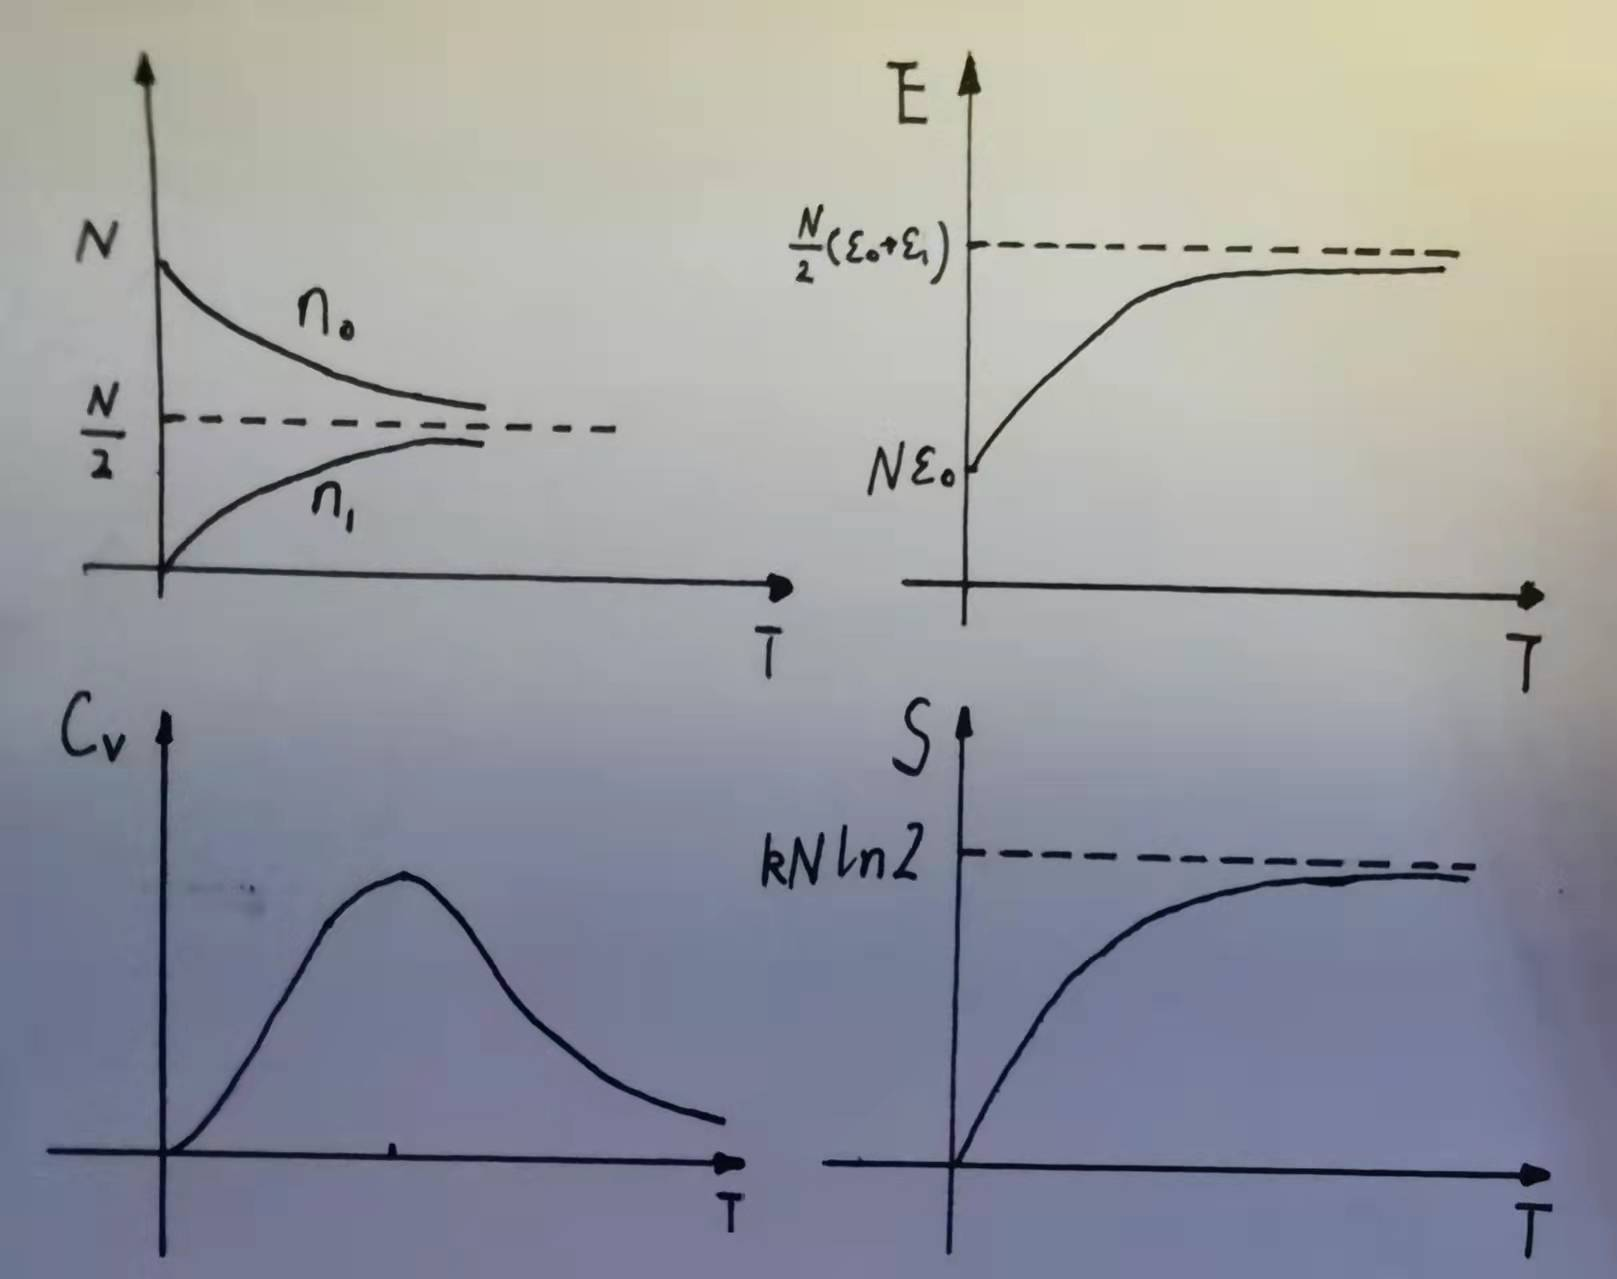
\includegraphics[width=8cm,height=8cm]{3_3.jpg}
\end{figure}
\section*{四、(本题25分)白矮星中心的温度为$T\approx10^7K$,可以把它看做是N个电子和$\frac{N}{2}$个
  氢核的系统。白矮星的费米温度$T_F\approx 10^9K$,因此其电子其他是高度简并的,可以把它看做是温度为绝对零度
  的理想费米气体。白矮星的存在是气体的简并压力与自引力达到暂态平衡的结果。如果这个气体是极端相对论的,则
  存在一个临界质量$M_c$,当白矮星的质量M大于临界质量$M_c$时,它将塌缩。只要电子是非相对论的,该费米气体
  就能抵抗引力塌缩而保持稳定。}
1.在极端相对论条件下,粒子的能量动量关系为$\varepsilon=pc$,证明在体积V,能量$\varepsilon\sim\varepsilon
  +d\varepsilon$的范围内,极端相对论粒子(自旋简并度为J)的量子态数为$g(\varepsilon)d\varepsilon=
  \frac{4\pi JV}{(ch)^3}\varepsilon^2d\varepsilon$;
\begin{equation*}
  \begin{aligned}
     & \Omega(\varepsilon)=\int dxdydzdp_xdp_ydp_z
    =V\int p^2sin\theta dpd\theta d\varphi
    =4\pi V\int_0^{\frac{\varepsilon}{c}} p^2dp
    =\frac{4\pi V\varepsilon^3}{3c^3}                                        \\
     & g(\varepsilon)=\frac{J}{h^3}\frac{d\Omega(\varepsilon)}{d\varepsilon}
    =\frac{4\pi JV\varepsilon^2}{(ch)^3}=\frac{8\pi V\varepsilon^2}{(ch)^3}
  \end{aligned}
\end{equation*}
2.在极端相对论情况下,利用费米-狄拉克统计导出电子气体在$T=0K$时的费米能量、内能和简并压。
\begin{equation*}
  \begin{aligned}
     & N=\int_0^{\varepsilon_F}g(\varepsilon)d\varepsilon
    =\frac{4\pi JV}{(ch)^3}\int_0^{\varepsilon_F}\varepsilon^2d\varepsilon
    =\frac{4\pi JV\varepsilon_F^3}{3(ch)^3}                                      \\
     & \varepsilon_F=(\frac{3N(ch)^3}{4\pi JV})^{\frac{1}{3}}
    =(\frac{3N}{8\pi V})^{\frac{1}{3}}ch                                         \\
     & \overline{E}=\int_0^{\varepsilon_F}\varepsilon g(\varepsilon)d\varepsilon
    =\frac{4\pi JV}{(ch)^3}\frac{\varepsilon_F^4}{4}
    =\frac{3}{4}chN(\frac{3N}{8\pi V})^\frac{1}{3}                               \\
     & P=-\frac{\partial\overline{E}}{\partial V}
    =\frac{chN}{8V}(\frac{3N}{\pi V})^\frac{1}{3}
  \end{aligned}
\end{equation*}
3.在非相对论条件下,当费米动量为$\frac{m_cc}{10}$时,求电子数密度。
\begin{equation*}
  \begin{aligned}
     & P_F=\frac{m_cc}{10},\quad\quad
    \varepsilon_F=\frac{p^2}{2mc}=\frac{m_cc^2}{200}                                  \\
     & n=\frac{2}{3}\varepsilon_F^\frac{3}{2}\times\frac{2\pi J(2m)^\frac{3}{2}}{h^3}
    =\frac{\pi m^3c^3}{375h^3}
  \end{aligned}
\end{equation*}
4.(选做3分)试导出白矮星临界质量$M_c$的表达式(忽略辐射)。
\section*{五、(本题20分)考虑由同种、无相互作用、非相对论的玻色子组成的气体,根据玻色-爱因斯坦
  分布解答以下问题:}
1.如果最低能级取$\varepsilon_0=0$,分析并给出化学势$\mu$的取值范围。
\begin{equation*}
  n_0=\frac{g_i}{e^{-\frac{\mu}{kT}}-1}\quad\quad
  n_0>0\quad\quad e^{-\frac{\mu}{kT}}>1,\quad\quad \mu<0
\end{equation*}
2.在系统的体积V和总粒子数N保持不变时,如果玻色气体是单原子分子组成的气体,证明
$\frac{\partial\mu}{\partial T}<0$;
\begin{equation*}
  \begin{aligned}
     & N=\int_0^\infty \frac{g(\varepsilon)d\varepsilon}{e^{\frac{\varepsilon-\mu}{kT}}-1}          \\
     & \frac{\partial\mu}{\partial T}=-\frac{\partial N}{\partial T}/\frac{\partial N}{\partial\mu}
    =-\frac{\int_0^\infty \frac{\varepsilon-\mu}{kT^2}
      \frac{e^\frac{\varepsilon-\mu}{kT}}{(e^\frac{\varepsilon-\mu}{kT}-1)^2}
      \sqrt{\varepsilon}d\varepsilon}
    {\int_0^\infty\frac{e^\frac{\varepsilon-\mu}{kT}}{(e^\frac{\varepsilon-\mu}{kT}-1)^2}
      \frac{\sqrt{\varepsilon}}{kT}d\varepsilon}<0
  \end{aligned}
\end{equation*}
3.导出基态能级$\varepsilon_0=0$及激发态能级$\varepsilon>0$上分布的粒子数与系统总粒子数N及温度T
的关系,进而说明该三维系统能否存在玻色-爱因斯坦凝聚?
\begin{equation*}
  \begin{aligned}
     & N_1=\int_0^\infty\frac{g(\varepsilon)d\varepsilon}{e^\frac{\varepsilon}{kT}-1}
    =\frac{2\pi VJ(2m)^\frac{3}{2}}{h^3}\int_0^\infty\frac{\sqrt{x}dx}{e^x-1}
    =2.612J(\frac{2\pi mkT}{h^2})^\frac{3}{2}=(\frac{T}{T_c})^\frac{3}{2}N            \\
     & N_0=N-N_1=(1-(\frac{T}{T_c})^\frac{3}{2})N
  \end{aligned}
\end{equation*}
能存在Bose-Einstein凝聚。\\
4.如何理解玻色-爱因斯坦凝聚是动量空间的凝聚?(定性说明即可)\\
参考公式:$\int_0^\infty\frac{\sqrt{x}dx}{e^x-1}=2.612\times\frac{\sqrt{\pi}}{2}=2.31$\\
凝聚到$\varepsilon=0$的粒子的动量、能量、熵都为0。

\end{document}